%!TEX program = xelatex
% 完整编译: xelatex -> biber/bibtex -> xelatex -> xelatex
\documentclass[lang=cn,11pt,a4paper]{elegantpaper}

\title{Fluent Mesh格式说明文档}
\author{IforeverYH}
\institute{\textcolor{red}{网格文件转换项目}}

\version{1.0}
\date{\zhtoday}

% 本文档命令
\usepackage{array}
\newcommand{\ccr}[1]{\makecell{{\color{#1}\rule{1cm}{1cm}}}}

\begin{document}

\maketitle

\begin{abstract}
  本文档为Fluent Mesh(.msh)\footnote{正文中用msh代替.msh,省略\textcolor{red}{.}}网格文件的格式说明文档。说明Fluent Mesh文件的数据存储格式。
\end{abstract}

\section{二维msh文本文件说明}

\subsection{文本文件示例}
以简单的 $2\times2$ 网格为例,其形状如图 \ref{2dMesh} 所示:

\begin{figure}[!htb]
\centering
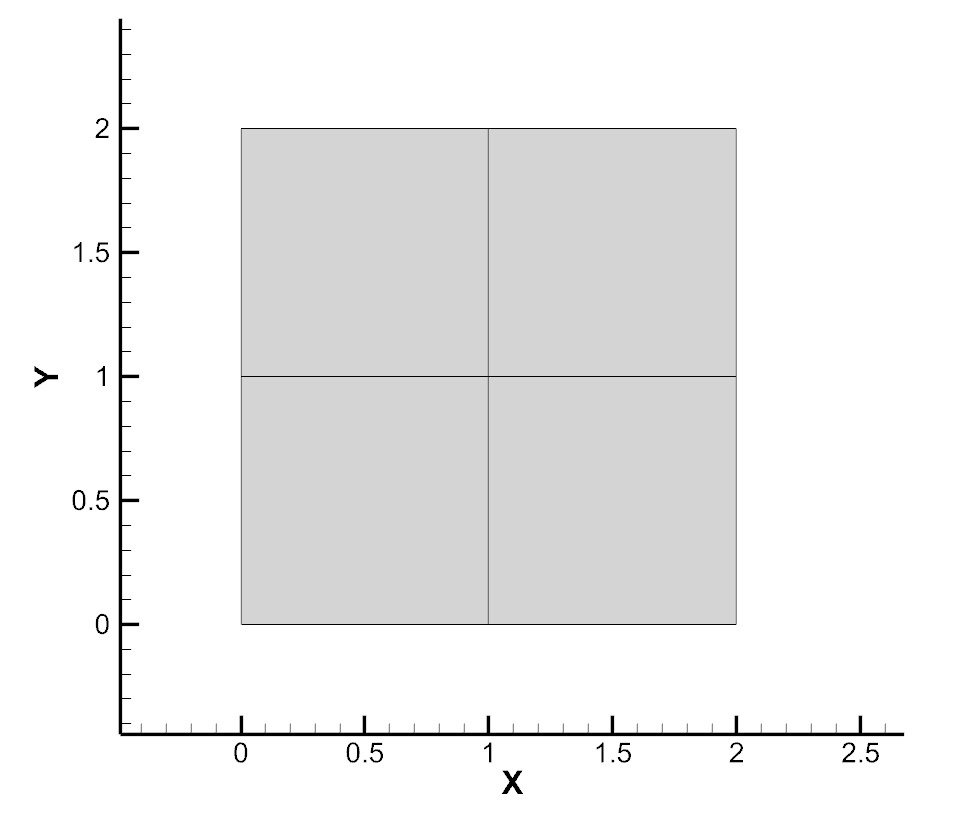
\includegraphics[width=0.6\textwidth]{2d.png}
\caption{二维网格示例}
\label{2dMesh}
\end{figure}

该网格对应的文本文件内容为:

\begin{lstlisting}
  (0 " Created by : Fluent_V6 Interface Vers. 18.2.0") % 版本信息
  (2 2) ---------------------------------------------- % 维度
  (0 "Node Section") --------------------------------- % 节点信息描述字段
  (10 (0 1 9 0 2)) ----------------------------------- % 节点信息总述字段
  (10 (5 1 9 1 2) ------------------------------------ % 节点头文字段
  (
  0 0
  1 0
  0 1
  1 1
  0 2
  1 2
  2 0
  2 1
  2 2
  ))
  (12 (0 1 4 0 0)) ------------------------------------ % Cells信息总述字段
  (12 (6 1 4 1 3))
  (13 (0 1 c 0 0))
  (0 "Interior faces of zone FLUID") ------------------ % 内部面信息描述字段
  (13 (7 1 4 2 2)(
  2 4 1 3
  4 3 1 2
  4 6 2 4
  8 4 3 4
  )
  )
  (0 "Faces of zone FAR") ----------------------------- % "far"面信息描述字段
  (13 (8 5 c 9 2)(
  1 2 1 0
  2 7 3 0
  3 1 1 0
  5 3 2 0
  7 8 3 0
  8 9 4 0
  6 5 2 0
  9 6 4 0
  )
  )
  (0 "Zone Sections") --------------------------------- % Zone信息描述字段
  (39 (6 fluid FLUID)())
  (39 (7 interior int_FLUID)())
  (39 (8 pressure-far-field FAR)()) 
\end{lstlisting}

文本文件格式按模块内容区分大类,一般分为以下内容:
\begin{enumerate}
  \item \textbf{描述字段}:出现在每个大类模块的第一行,为下面内容的大类信息;
  \item \textbf{总述字段}:出现在描述字段之后,对内容进行总述(相当于头文字段的总结),常见于节点,单元信息等模块;
  \item \textbf{头文字段}:描述该部分的内容的类型,成员起止编号,成员类型等信息;
  \item \textbf{具体内容}:在头文字段之后,为网格各类模块的具体信息,包括节点坐标,几何关系等内容。
\end{enumerate}

\subsection{描述字段}\label{Comment}
\begin{lstlisting}
  {描述字段格式}:(0 "comment text")
  {格式解释}:0为指令标号;
             "comment text"为描述文本。
\end{lstlisting}

\subsection{维度}\label{Dimensions}
\begin{lstlisting}
  {维度格式}:(2 n)
  {格式解释}:2为指令标号;
             第二个数字为维数,2表示2维、3表示3维。 
\end{lstlisting}

\subsection{Nodes 节点}\label{Nodes}
\begin{lstlisting}
  {节点格式}:(10 (zone-id first-index last-index type ND)(x1 y1 z1  x2 y2 z2... ))
  {格式解释}:10为指令标号;
             zone-id为区域编号;
             first-index为该区域第一个成员的编号;
             last-index为该区域最后一个成员的编号;
             type为节点类型;
             ND为维度;
             (x y z)为每个节点的坐标(10进制)。
\end{lstlisting}

\subsubsection{使用说明}
\begin{enumerate}
  \item \textbf{如果zone-id = 0}:first-index = 1,last-index为节点总数,type置0,ND后面不跟坐标数据。此时相当于对nodes的整体说明,即总述字段;
  \item \textbf{如果zone-id > 0}:表示结构体中的nodes属于编号zone-id的zone区域。此时first-index和last-index为该zone区域的节点起止编号,节点的坐标信息在ND后的()内;
  \item \textbf{如果ND = 2}:节点数据不显示z坐标。
\end{enumerate}

\subsubsection{type设置规则}\label{node-type}
\begin{enumerate}[label=\arabic*).]
  \item \lstinline{0}: "virtual" nodes -- 虚拟节点;
  \item \lstinline{1}: no(any) type -- 通用型;
  \item \lstinline{2}: boundary nodes -- 边界节点。
\end{enumerate}

\subsection{Cells 单元}\label{Cells}
\begin{lstlisting}
  {单元格式}:(12 (zone-id first-index last-index type element-type)())
  {格式解释}:12为指令标号;
             zone-id为区域编号;
             first-index为该区域第一个成员的编号;
             last-index为该区域最后一个成员的编号;
             type为单元物理属性;
             element-type为单元类型;
             ()仅当element-type = 0时使用。
\end{lstlisting}

\subsubsection{使用说明}
\begin{enumerate}
  \item \textbf{如果zone-id = 0}:first-index = 1,last-index为单元总数(若last-index = 0则表示文件中无cell),
                                  type置0,计算时Fluent会忽略type = 0的区域(死区),element-type不显示(或置0)。此时相当于对cells的整体说明,即总述字段;
  \item \textbf{如果zone-id > 0}:表示结构体中的cells属于编号zone-id的zone区域。type = 1 为流体,type = 17(0x11)为固体。
\end{enumerate}

\textbf{特别注意}:如果单元类型为混合型(element-type = 0),则列出每个单元的类型。此时单元格式后接一对()。
具体可见下面的例子,区域9有61个单元,其中前3个为三角单元,紧接两个六面体单元,等等。
\begin{lstlisting}
  (12 (9 1 3d 1 0)(
  1 1 1 3 3 1 1 3 1
  ...
  ))
\end{lstlisting}

\subsubsection{element-type设置规则}\label{element-type}
\begin{enumerate}[label=\arabic*).]
  \item \lstinline{0}: mixed;
  \item \lstinline{1}: triangular -- 三角形;
  \item \lstinline{2}: tetrahedral -- 四面体;
  \item \lstinline{3}: quadrilateral -- 四边形;
  \item \lstinline{4}: hexahedral -- 六面体;
  \item \lstinline{5}: pyramid -- 四棱锥(金字塔);
  \item \lstinline{6}: wedge -- 楔形;
  \item \lstinline{7}: polyhedral -- 多面体。
\end{enumerate}

\subsection{Faces 面}\label{Faces}
\begin{lstlisting}
  {面格式}:(13 (zone-id first-index last-index bc-type face-type)())
  {格式解释}:13为指令标号;
             zone-id为区域编号;
             first-index为该区域第一个成员的编号;
             last-index为该区域最后一个成员的编号;
             bc-type为边界条件;
             face-type为面类型;
             ()内存放点、面、单元的关系。
\end{lstlisting}

\subsubsection{使用说明}
\begin{enumerate}
  \item \textbf{如果zone-id = 0}:first-index = 1,last-index为面总数,bc-type不显示(或置0)。此时相当于对faces的整体说明,即总述字段;
  \item \textbf{如果zone-id > 0}:表示结构体中的faces属于编号zone-id的zone区域,面数据的信息在随后的()内。
\end{enumerate}

\subsubsection{bc-type设置规则}\label{bc-type}
\begin{enumerate}[label=\arabic*).]
  \item \lstinline{2(Ox2)}: interior;
  \item \lstinline{3(Ox3)}: wall;
  \item \lstinline{4(Ox4)}: pressure-inlet, inlet-vent, intake-fan;
  \item \lstinline{5(Ox5)}: pressure-outlet, outlet-vent, exhaust-fan;
  \item \lstinline{7(Ox7)}: symmetry;
  \item \lstinline{8(Ox8)}: periodic-shadow;
  \item \lstinline{9(Ox9)}: pressure-far-field;
  \item \lstinline{10(Oxa)}: velocity-inlet;
  \item \lstinline{12(Oxc)}: periodic; 
  \item \lstinline{14(Oxe)}: fan, porous-jump, radiztor;
  \item \lstinline{20(Ox14)}: mass-flow-inlet;
  \item \lstinline{24(Ox18)}: Interface;
  \item \lstinline{31(Ox1f)}: parent(hanging node);
  \item \lstinline{36(Ox24)}: outflow;
  \item \lstinline{37(Ox25)}: axis.
\end{enumerate}

\textbf{注意}:非共形网格相交的交界面被存放在一个单独的面区域中。这些面区域的bc-type增加了1000(例如bc-type = 1003是wall);这里所写的边界条件的标号要转16进制。

\subsubsection{face-type设置规则}\label{face-type}
\begin{enumerate}[label=\arabic*).]
  \item \lstinline{0}: mixed;
  \item \lstinline{2}: linear;
  \item \lstinline{3}: triangular;
  \item \lstinline{4}: quadrilateral;
  \item \lstinline{5}: polygonal.
\end{enumerate}

\subsubsection{点、面、单元关系格式}
\begin{lstlisting}
  {面关系格式}:(n0 n1 n2 c0 c1)
  {格式解释}:n*表示节点编号,其最大标号与face-type相关;
             c*表示face的邻近cell编号,c0按右手法则确定,c1在face的另一边;
\end{lstlisting}

对于二维情况,假设存在一个指向平面外的$\overrightarrow{k}$,通过$\overrightarrow{k}\times\overrightarrow{r}$来确定c0;在边界处c0或c1为0。

当网格为混合类型(face-type = 0)或多边形类型(face-type = 5),每一行说明面的语句应以节点数目开头:
\begin{lstlisting}
  (x n0 n1 ... nf c0 c1) 
\end{lstlisting}

\subsection{Face Tree}\label{Face-Tree}
\begin{lstlisting}
  {区域格式}:(59 (face-id0 face-id1 parent-zone-id child-zone-id)
                 (number-of-kids kid-id-0 kid-id-1 ... kid-id-n))
  {格式解释}:59为指令标号;
             face-id0为区域第一个父级面的编号;
             face-id1为区域最后一个父级面的编号;
             parent-zone-id为父级面所在区域id;
             child-zone-id为子级面所在区域id;
             number-of-kids为子级面的数量;
             kid-id-n为子级面的编号。
\end{lstlisting}

\subsection{Cell Tree}\label{Cell-Tree}
\begin{lstlisting}
  {区域格式}:(58 (cell-id0 cell-id1 parent-zone-id child-zone-id)
                 (number-of-kids kid-id-0 kid-id-1 ... kid-id-n))
  {格式解释}:58为指令标号;
             cell-id0为区域第一个父级单元的编号;
             cell-id1为区域最后一个父级单元的编号;
             parent-zone-id为父级单元所在区域id;
             child-zone-id为子级单元所在区域id;
             number-of-kids为子级单元的数量;
             kid-id-n为子级单元的编号。
\end{lstlisting}

\subsection{Zone 区域}\label{Zone}
\begin{lstlisting}
  {区域格式}:(39 (zone-id zone-type zone-name domain-id)())
  {格式解释}:39为指令标号;
             zone-id为区域编号(10进制);
             zone-type为区域类型(一般是指边界条件);
             zone-name为区域名称;
             domain-id(ICEM输出的msh一般是忽略不写);
             ()空。
\end{lstlisting}

\subsubsection{zone-type设置规则}\label{zone-type}
\begin{table}[!htb]
  \centering
  \caption{可用的zone-type种类}
  \begin{tabular}{*{3}{l}}
   \hline
   \texttt{degassing}       & \texttt{exhaust-fan}   & \texttt{fan} \\
   \texttt{fluid}           & \texttt{geometry}      & \texttt{inlet-vent} \\
   \texttt{intake-fan}      & \texttt{interface}     & \texttt{interior} \\
   \texttt{internal}        & \texttt{mass-flow-inlet}          & \texttt{outflow} \\
   \texttt{outlet-vent}     & \texttt{parent-face}   & \texttt{porous-jump} \\
   \texttt{pressure-far-field}         & \texttt{pressure-inlet}     & \texttt{pressure-outlet} \\
   \texttt{radiator}        & \texttt{solid}         & \texttt{symmetry} \\
   \texttt{velocity-inlet}  & \texttt{wall}          & \texttt{wrapper} \\
   \hline
  \end{tabular}
\end{table}

\section{三维msh文本文件示例}

三维网格以 $2\times2\times2$ 立方体为例,边长为2,其形状如图 \ref{3dMesh} 所示:
\begin{figure}[!htb]
\centering
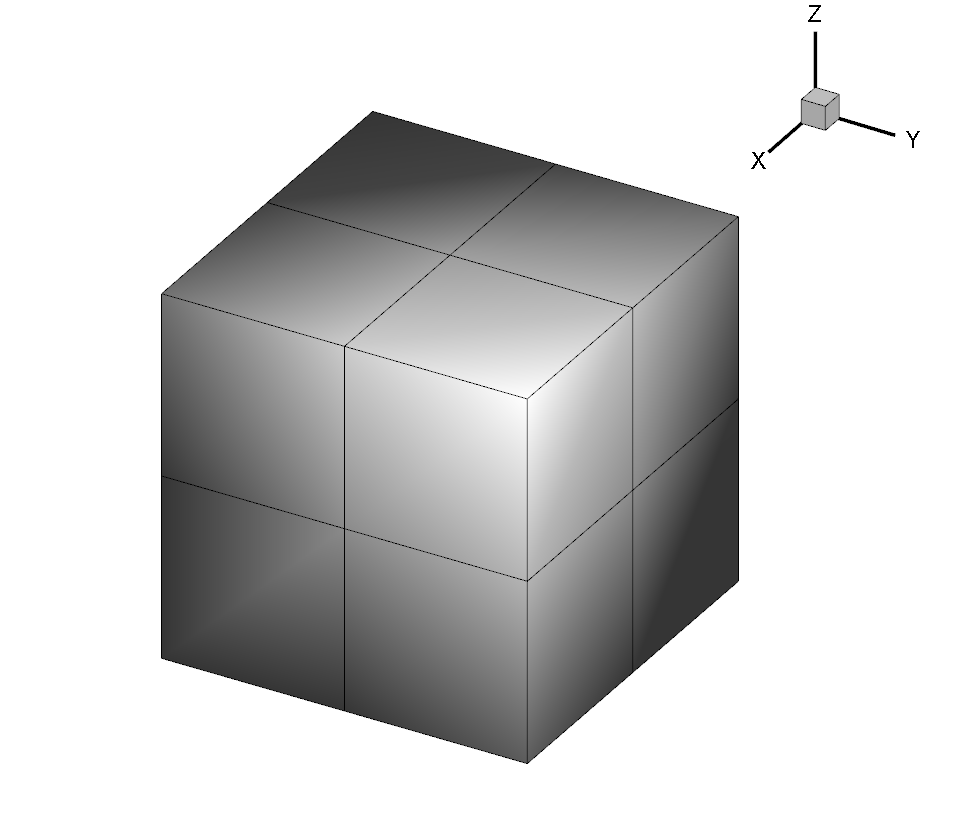
\includegraphics[width=0.5\textwidth]{3d.png}
\caption{三维网格示例}
\label{3dMesh}
\end{figure}

该网格对应的文本文件内容为:

\begin{lstlisting}
  (0 " Created by : Fluent_V6 Interface Vers. 18.2.0")
  (2 3)
  (0 "Node Section")
  (10 (0 1 1b 0 3))
  (10 (5 1 1b 1 3)
  (
  0 0 0
  1 0 0
  0 1 0
  1 1 0
  0 0 1
  1 0 1
  0 1 1
  1 1 1
  0 0 2
  1 0 2
  0 1 2
  1 1 2
  0 2 0
  1 2 0
  0 2 1
  1 2 1
  0 2 2
  1 2 2
  2 0 0
  2 1 0
  2 0 1
  2 1 1
  2 0 2
  2 1 2
  2 2 0
  2 2 1
  2 2 2
  ))
  (12 (0 1 8 0 0))
  (12 (6 1 8 1 4))
  (13 (0 1 24 0 0))
  (0 "Interior faces of zone FLUID")
  (13 (7 1 c 2 4)(
  3 4 8 7 1 3
  2 6 8 4 1 5
  5 7 8 6 1 2
  7 8 c b 2 4
  6 a c 8 2 6
  4 8 10 e 3 7
  7 f 10 8 3 4
  8 c 12 10 4 8
  4 14 16 8 5 7
  6 8 16 15 5 6
  8 16 18 c 6 8
  8 10 1a 16 7 8
  )
  )
  (0 "Faces of zone FAR")
  (13 (1 d 24 9 4)(
  1 3 7 5 1 0
  5 7 b 9 2 0
  3 d f 7 3 0
  7 f 11 b 4 0
  1 5 6 2 1 0
  5 9 a 6 2 0
  2 6 15 13 5 0
  6 a 17 15 6 0
  1 2 4 3 1 0
  3 4 e d 3 0
  2 13 14 4 5 0
  4 14 19 e 7 0
  13 15 16 14 5 0
  15 17 18 16 6 0
  14 16 1a 19 7 0
  16 18 1b 1a 8 0
  d e 10 f 3 0
  f 10 12 11 4 0
  e 19 1a 10 7 0
  10 1a 1b 12 8 0
  9 b c a 2 0
  b 11 12 c 4 0
  a c 18 17 6 0
  c 12 1b 18 8 0
  )
  )
  (0 "Zone Sections")
  (39 (6 fluid FLUID)())
  (39 (7 interior int_FLUID)())
  (39 (1 pressure-far-field FAR)()) ------------ %自定义编号1
\end{lstlisting}

\section{Mesh with Hanging Nodes(搭接网格)}

这里直接给出Fluent用户手册中的例子。
\begin{figure}[!htb]
  \centering
  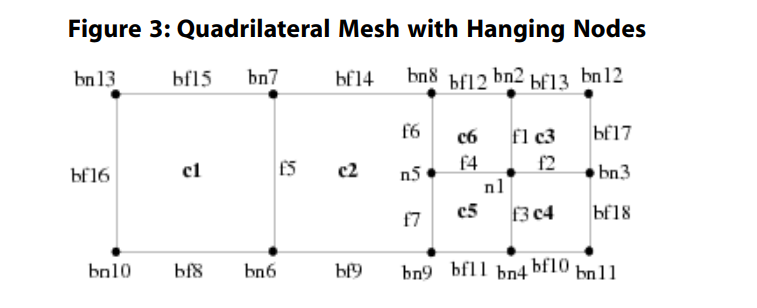
\includegraphics[width=0.6\textwidth]{hanging.png}
  \caption{网格示例}
  \label{hanging}
  \end{figure}
\begin{lstlisting}
  (0 "Grid:")
  (0 "Dimensions:")
  (2 2)
  (12 (0 1 7 0))
  (13 (0 1 16 0))
  (10 (0 1 d 0 2))
  (12 (7 1 6 1 3))
  (12 (1 7 7 20 3))
  (58 (7 7 1 7)(
  4 6 5 4 3))
  (13 (2 1 7 2 2)(
  1 2 6 3 
  1 3 3 4 
  1 4 4 5 
  1 5 5 6 
  6 7 1 2 
  5 8 2 6 
  9 5 2 5))
  (13 (3 8 b 3 2)(
  a 6 1 0 
  6 9 2 0 
  4 b 4 0 
  9 4 5 0))
  (13 (4 c f 3 2)(
  2 8 6 0 
  c 2 3 0 
  8 7 2 0 
  7 d 1 0))
  (13 (5 10 10 a 2)(
  d a 1 0))
  (13 (6 11 12 24 2)(
  3 c 3 0 
  b 3 4 0))
  (13 (b 13 13 1f 2)(
  c 8 7 0))
  (13 (a 14 14 1f 2)(
  b c 7 0))
  (13 (9 15 15 1f 2)(
  9 b 7 0))
  (13 (8 16 16 1f 2)(
  9 8 2 7))
  (59 (13 13 b 4)(
  2 d c))
  (59 (14 14 a 6)(
  2 12 11))
  (59 (15 15 9 3)(
  2 b a))
  (59 (16 16 8 2)(
  2 7 6))
  (10 (1 1 d 1 2)
  (
  2.50000000e+00 5.00000000e-01
  2.50000000e+00 1.00000000e+00
  3.00000000e+00 5.00000000e-01
  2.50000000e+00 0.00000000e+00
  2.00000000e+00 5.00000000e-01
  1.00000000e+00 0.00000000e+00
  1.00000000e+00 1.00000000e+00
  2.00000000e+00 1.00000000e+00
  2.00000000e+00 0.00000000e+00
  0.00000000e+00 0.00000000e+00
  3.00000000e+00 0.00000000e+00
  3.00000000e+00 1.00000000e+00
  0.00000000e+00 1.00000000e+00))
\end{lstlisting}

需要注意的事项:
\begin{enumerate}
  \item hanging node存在时要注意相应cell和face头文字段的内容。举例来说,在上述示例中可以认为在细网格区外存在一个大cell,包裹4个小cells;
  \item 通过Star CCM+的切割体网格生成器(Trimmed Mesher)生成的网格,转换为Fluent msh后,face-type(面类型)被识别为polygonal(多边形),element-type(单元类型)被识别为polyhedral(多面体)。
\end{enumerate}


\section{附录}

\subsection{Index检索}
检索列表列出.msh的所有可用的指令标号,需要用到的有索引指示。
\begin{enumerate}[label=\arabic*).]
  \item \lstinline{0}: Comment\upref{Comment}, -optional;
  \item \lstinline{1}: Header, -optional;
  \item \lstinline{2}: Dimensions\upref{Dimensions}, -optional;
  \item \lstinline{10}: Nodes\upref{Nodes}, -required;
  \item \lstinline{11}: Edges, -optional;
  \item \lstinline{12}: Cells\upref{Cells}, -required;
  \item \lstinline{13}: Faces\upref{Faces}, -required;
  \item \lstinline{18}: Periodic Shadow Faces, -required with periodic boundaries;
  \item \lstinline{39 or 45}: Zone\upref{Zone}, -required;(当有边界条件时必须用39)
  \item \lstinline{58}: Cell Tree\upref{Cell-Tree}, only for grids with hanging-node adaption;
  \item \lstinline{59}: Face Tree\upref{Face-Tree}, only for grids with hanging-node adaption;
  \item \lstinline{61}: Interface Face Parents, only for grids with non-conformal Interfaces.
\end{enumerate}

\subsection{X-type设置检索}
\begin{enumerate}
  \item node-type\upref{node-type};
  \item element-type\upref{element-type};
  \item bc-type\upref{bc-type};
  \item face-type\upref{face-type};
  \item zone-type\upref{zone-type}.
\end{enumerate}

\end{document}